\chapter{Pernyataan Matematis Formal}
\begin{outcome}
\begin{itemize}
\item Menetapkan notasi matematis yang diperlukan
\item Memahami hasil-hasil struktural yang berkaitan dengan program linier
\item Mengembangkan intuisi tentang alasan hasil-hasil tersebut berlaku
\end{itemize}
\end{outcome}

\begin{quote}
\itshape Anda telah menyelesaikan masalah toko roti secara grafis: Anda memeriksa beberapa titik sudut dan memilih yang terbaik. Namun, daerah layak memuat tak terhingga banyak titik. Bagaimana Anda dapat \emph{mengetahui} bahwa rencana yang lebih baik tidak tersembunyi di tengah daerah, atau di suatu bagian sisi yang tidak pernah Anda periksa? Dalam dua dimensi, sebuah gambar cukup meyakinkan. Model produksi nyata memiliki ribuan variabel dan tidak dapat digambarkan. Bab ini mengganti gambar dengan bukti: argumen singkat yang memastikan, untuk seterusnya, bahwa memeriksa titik-titik sudut saja sudah cukup.
\end{quote}

Dalam bab ini, kita memformalkan sebagian konsep matematika mengenai program linier. Kita mendefinisikan beberapa notasi, lalu menyatakan dan membuktikan sejumlah teorema.

\begin{warn}
Dalam bagian ini, kita menyajikan bukti matematis yang ketat bagi beberapa hasil. Untuk buku ini, Anda tidak perlu mampu mereproduksi bukti-bukti tersebut. Namun, cobalah memahami konsepnya dan membentuk gambaran visual dalam benak tentang alasan hasil-hasil tersebut berlaku.
\end{warn}

\section{Dasar-Dasar Matematika}\label{sec:math-preliminaries}

\subsection{Vektor dan Sifat-Sifatnya}

\textbf{Vektor:}  
Vektor adalah objek matematis yang menyatakan sebuah titik dalam ruang atau suatu arah. Dalam ruang riil berdimensi \(n\) (\(\mathbb{R}^n\)), vektor \(\mathbf{v}\) ditulis sebagai daftar terurut berisi \(n\) elemen:  
\[
\mathbf{v} = (v_1, v_2, \dots, v_n).
\]  
Vektor dapat ditulis dalam dua bentuk: sebagai vektor baris \([v_1, v_2, \dots, v_n]\) atau sebagai vektor kolom:
\[
\mathbf{v} = \begin{bmatrix} v_1 \\ v_2 \\ \vdots \\ v_n \end{bmatrix}.
\]  
Dalam program linier, vektor digunakan untuk menyatakan variabel, kendala, dan arah dalam masalah optimisasi.

\medskip  
\textbf{Operasi Vektor:}  
Operasi vektor merupakan unsur dasar program linier yang memungkinkan kita memanipulasi variabel keputusan dan kendala.

\begin{description}
    \item[Penjumlahan:]  
    Vektor-vektor dengan dimensi yang sama dapat dijumlahkan per komponen. Sebagai contoh, jika \(\mathbf{v} = (2, 3)\) dan \(\mathbf{u} = (3, 2)\), jumlahnya adalah:  
    \[
    \mathbf{v} + \mathbf{u} = (2+3, 3+2) = (5, 5).
    \]  
    Operasi ini digunakan untuk memodelkan sistem yang menggabungkan kontribusi beberapa variabel.

    \item[Perkalian Skalar:]  
    Sebuah vektor dapat diskalakan dengan mengalikannya dengan skalar (konstanta). Sebagai contoh, jika \(k = 2\) dan \(\mathbf{v} = (2, 3)\), maka:
    \[
    k\mathbf{v} = (2 \cdot 2, 3 \cdot 2) = (4, 6).
    \]  
    Perkalian skalar mengubah besar vektor sambil mempertahankan arahnya, sebuah konsep penting saat menskalakan kendala atau objektif dalam program linier.

    \item[Hasil Kali Dalam (Titik):]  
    Hasil kali titik dua vektor \(\mathbf{v}\) dan \(\mathbf{u}\) yang berukuran sama dihitung sebagai:
    \[
    \mathbf{v} \cdot \mathbf{u} = \sum_{i=1}^n v_i u_i.
    \]  
    Sebagai contoh, jika \(\mathbf{v} = (2, 3)\) dan \(\mathbf{u} = (3, 2)\), maka:
    \[
    \mathbf{v} \cdot \mathbf{u} = 2 \cdot 3 + 3 \cdot 2 = 10.
    \]  
    Hasil kali titik digunakan untuk mendefinisikan kendala dan fungsi objektif dalam program linier karena menyatakan jumlah berbobot dari variabel-variabel.
\end{description}

\subsection{Kombinasi Linier dan Konsep Terkait}

\textbf{Kombinasi Linier:}  
Vektor \(\mathbf{u}\) merupakan kombinasi linier dari vektor-vektor \(\mathbf{v}^1, \mathbf{v}^2, \dots, \mathbf{v}^k\) jika:
\[
\mathbf{u} = \sum_{i=1}^k \lambda_i \mathbf{v}^i,
\]
dengan \(\lambda_1, \lambda_2, \dots, \lambda_k\) berupa skalar. Jika semua skalar tak negatif (\(\lambda_i \geq 0\)), kombinasi tersebut disebut \emph{kombinasi linier tak negatif}. Kombinasi linier digunakan dalam program linier untuk menyatakan solusi layak sebagai jumlah kontribusi variabel.

\begin{definition}{Kebebasan Linier}{}
Suatu himpunan vektor \( \{ \mathbf{v}^1, \mathbf{v}^2, \dots, \mathbf{v}^k \} \subseteq \mathbb{R}^n \) disebut \emph{bebas linier} jika satu-satunya solusi bagi persamaan
\[
\lambda_1 \mathbf{v}^1 + \lambda_2 \mathbf{v}^2 + \dots + \lambda_k \mathbf{v}^k = \mathbf{0}
\]
adalah \( \lambda_1 = \lambda_2 = \dots = \lambda_k = 0 \).  

Secara ekuivalen, tidak ada vektor dalam himpunan tersebut yang dapat ditulis sebagai kombinasi linier dari vektor-vektor lainnya.
\end{definition}

\textbf{Contoh:}
\begin{itemize}
    \item Vektor \( \begin{bmatrix}1\\0\end{bmatrix} \) dan \( \begin{bmatrix}0\\1\end{bmatrix} \) dalam \( \mathbb{R}^2 \) bebas linier.
    \item Vektor \( \begin{bmatrix}1\\2\end{bmatrix} \) dan \( \begin{bmatrix}2\\4\end{bmatrix} \) bergantung linier karena vektor kedua merupakan kelipatan skalar dari vektor pertama.
\end{itemize}

\vspace{1em}

\begin{definition}{Kebebasan Linier Baris atau Kolom}{}
Misalkan \( A \in \mathbb{R}^{m \times n} \) adalah sebuah matriks.

\begin{itemize}
  \item Baris-baris \( A \) disebut \emph{bebas linier} jika tidak ada baris yang dapat ditulis sebagai kombinasi linier dari baris-baris lainnya.
  
  \item Kolom-kolom \( A \) disebut \emph{bebas linier} jika tidak ada kolom yang dapat ditulis sebagai kombinasi linier dari kolom-kolom lainnya.
  
  \item Dalam kedua kasus, vektor-vektor tersebut bebas linier jika satu-satunya solusi sistem homogen \( A \mathbf{x} = \mathbf{0} \) (atau \( A^\top \mathbf{y} = \mathbf{0} \)) adalah solusi trivial \( \mathbf{x} = \mathbf{0} \) (atau \( \mathbf{y} = \mathbf{0} \)).
\end{itemize}
\end{definition}

\textbf{Contoh:}
\begin{itemize}
    \item Matriks \( A = \begin{bmatrix}1 & 0 \\ 0 & 1\end{bmatrix} \) memiliki baris dan kolom yang bebas linier.
    \item Matriks \( A = \begin{bmatrix}1 & 2 \\ 2 & 4\end{bmatrix} \) memiliki baris dan kolom yang bergantung linier; baris kedua adalah dua kali baris pertama, dan kolom kedua adalah dua kali kolom pertama.
\end{itemize}

\vspace{1em}

\begin{definition}{Rank Matriks}{}
Misalkan \( A \in \mathbb{R}^{m \times n} \). Besaran \emph{rank} dari \( A \), yang dinyatakan dengan \( \operatorname{rank}(A) \), adalah jumlah maksimum baris atau kolom \( A \) yang bebas linier.

Secara ekuivalen, \( \operatorname{rank}(A) \) adalah:
\begin{itemize}
  \item dimensi ruang baris \( A \),
  \item dimensi ruang kolom \( A \),
  \item jumlah kolom pivot dalam bentuk eselon baris tereduksi \( A \),
  \item bilangan bulat terbesar \( r \) sedemikian sehingga \( A \) memiliki submatriks \( r \times r \) dengan determinan tak nol.
\end{itemize}
\end{definition}

\textbf{Contoh:}
\begin{itemize}
    \item Matriks \( A = \begin{bmatrix}1 & 2 \\ 3 & 4\end{bmatrix} \) memiliki rank penuh 2.
    \item Matriks \( A = \begin{bmatrix}1 & 2 \\ 2 & 4\end{bmatrix} \) memiliki rank 1 karena baris kedua merupakan kelipatan baris pertama.
\end{itemize}

\vspace{1em}

\begin{definition}{Kendala yang Bebas Linier}{}
Misalkan \( A \mathbf{x} \leq \mathbf{b} \) adalah sistem pertidaksamaan linier dengan setiap kendala bersesuaian dengan baris \( A_i \mathbf{x} \leq b_i \). Sebuah subhimpunan kendala tersebut disebut \emph{bebas linier} pada titik \( \mathbf{x} \in \mathbb{R}^n \) jika himpunan vektor baris \( \{ A_i : A_i \mathbf{x} = b_i \} \) (yakni kendala yang aktif pada \( \mathbf{x} \)) bebas linier.

Secara ekuivalen, kendala aktif pada \( \mathbf{x} \) bebas linier jika matriks \( A_I \), yang dibentuk dengan menumpuk baris-baris aktif, memenuhi
\[
\operatorname{rank}(A_I) = |I|,
\]
dengan \( I := \{ i : A_i \mathbf{x} = b_i \} \).
\end{definition}

\textbf{Contoh:}
\begin{itemize}
    \item Misalkan \( A \mathbf{x} \leq \mathbf{b} \) adalah sistem:
    \[
    \begin{aligned}
    x_1 &\leq 1 \\
    x_2 &\leq 1 \\
    x_1 + x_2 &\leq 2
    \end{aligned}
    \]
    Pada \( \mathbf{x} = (1, 1) \), ketiga kendala aktif. Dua kendala pertama memiliki vektor baris \( [1,0] \) dan \( [0,1] \), yang bebas linier. Kendala ketiga adalah \( [1,1] \), yang merupakan kombinasi linier dari dua kendala pertama. Jadi, hanya dua kendala aktif yang bebas linier.
    
    \item Sebaliknya, untuk sistem:
    \[
    \begin{aligned}
    x_1 &\leq 0 \\
    x_2 &\leq 0
    \end{aligned}
    \]
    pada titik \( \mathbf{x} = (0,0) \), kedua kendala aktif dan baris-barisnya \( [1,0] \), \( [0,1] \) bebas linier. Jadi, kendala aktif pada titik tersebut bebas linier.
\end{itemize}

\section{Bukti Aljabar -- Solusi Optimal Ada pada Titik Sudut}\label{sec:algebraic-vertex-proof}

\begin{definition}{Titik Sudut}{}
Misalkan \( P = \{ \mathbf{x} \in \mathbb{R}^n : A \mathbf{x} \leq \mathbf{b} \} \) adalah sebuah polihedron.  
Titik \( \mathbf{x} \in P \) disebut \emph{titik sudut} (atau \emph{titik pojok}) \( P \) jika merupakan solusi tunggal bagi suatu sistem yang terdiri atas \( n \) kendala bebas linier yang aktif pada \( \mathbf{x} \).  
Dengan kata lain, \( \mathbf{x} \) merupakan titik sudut jika terdapat subhimpunan \( I \subseteq \{1, \dots, m\} \) sedemikian sehingga:
\begin{itemize}
  \item \( A_i \mathbf{x} = b_i \) untuk semua \( i \in I \),
  \item Baris-baris \( \{ A_i : i \in I \} \) bebas linier,
  \item \( |I| = n \).
\end{itemize}
\end{definition}

\begin{theorem}{}{}
Misalkan \( \max \{ \mathbf{c}^\top \mathbf{x} : A \mathbf{x} \leq \mathbf{b} \} \) adalah program linier dengan daerah layak \( P \) yang tak kosong dan terbatas.  
Jika solusi optimal ada, maka terdapat solusi optimal yang merupakan titik sudut \( P \).
\end{theorem}

\begin{proof}
Misalkan \( \mathbf{x}^* \in P \) adalah solusi optimal. Jika \( \mathbf{x}^* \) merupakan titik sudut, pembuktian selesai. Jadi, misalkan \( \mathbf{x}^* \) \emph{bukan} titik sudut. Kita menunjukkan cara menghasilkan solusi optimal lain dengan himpunan kendala aktif bebas linier yang lebih besar secara ketat; pengulangan argumen ini menghasilkan titik sudut yang optimal.

Definisikan himpunan indeks kendala aktif pada \( \mathbf{x}^* \) sebagai
\[
I := \{ i \in \{1, \dots, m\} : A_i \mathbf{x}^* = b_i \},
\]
dengan \( A_i \) sebagai baris ke-$i$ dari \( A \). Misalkan \( A_I \) adalah submatriks \( A \) yang terdiri atas baris-baris berindeks \( I \).

Karena \( \mathbf{x}^* \) bukan titik sudut, kendala aktif tidak memuat \( n \) baris bebas linier: \( \operatorname{rank}(A_I) < n \). Oleh sebab itu, sistem homogen \( A_I \mathbf{d} = 0 \) mempunyai solusi tak nol \( \mathbf{d} \in \mathbb{R}^n \setminus \{0\} \).

Perhatikan garis \( \mathbf{x}(t) := \mathbf{x}^* + t \mathbf{d} \) untuk \( t \in \mathbb{R} \) yang kecil. Untuk semua \( i \in I \), berlaku:
\[
A_i \mathbf{x}(t) = A_i \mathbf{x}^* + t A_i \mathbf{d} = b_i + 0 = b_i,
\]
sehingga kendala aktif tetap aktif di sepanjang garis tersebut.

Untuk setiap \( i \notin I \), berlaku \( A_i \mathbf{x}^* < b_i \). Karena \( A_i \mathbf{x}(t) = A_i \mathbf{x}^* + t \, A_i \mathbf{d} \) bergantung secara kontinu pada \( t \), kita dapat memilih \( \varepsilon > 0 \) yang cukup kecil sehingga \( A_i \mathbf{x}(t) \leq b_i \) untuk semua \( t \in [-\varepsilon, \varepsilon] \) dan semua \( i \notin I \). Jadi, untuk \( t \) yang kecil, \( \mathbf{x}(t) \in P \).

Sekarang definisikan nilai objektif di sepanjang garis ini: 
\[
z(t) := \mathbf{c}^\top \mathbf{x}(t) = \mathbf{c}^\top \mathbf{x}^* + t \cdot (\mathbf{c}^\top \mathbf{d}).
\]

\begin{itemize}
\item Jika \( \mathbf{c}^\top \mathbf{d} > 0 \), maka untuk \( t > 0 \) yang kecil, \( \mathbf{x}(t) \in P \) dan \( \mathbf{c}^\top \mathbf{x}(t) > \mathbf{c}^\top \mathbf{x}^* \), yang bertentangan dengan keoptimalan \( \mathbf{x}^* \).
\item Jika \( \mathbf{c}^\top \mathbf{d} < 0 \), maka untuk \( t < 0 \) yang kecil kita memperoleh pertentangan yang sama.
\end{itemize}

Jadi, \( \mathbf{c}^\top \mathbf{d} = 0 \), sehingga setiap titik \( \mathbf{x}(t) \) yang terletak dalam \( P \) juga optimal. Di sinilah keterbatasan \( P \) digunakan: karena \( P \) terbatas, seluruh garis \( \{ \mathbf{x}(t) : t \in \mathbb{R} \} \) tidak mungkin termuat dalam \( P \), sehingga himpunan \( \{ t \geq 0 : \mathbf{x}(t) \in P \} \) merupakan interval tertutup dan terbatas \( [0, t^+] \). Pada \( t = t^+ \), suatu kendala \( j \notin I \) menjadi aktif: \( A_j \mathbf{x}(t^+) = b_j \). Perhatikan bahwa \( A_j \mathbf{d} \neq 0 \), sebab jika tidak, \( A_j \mathbf{x}(t) \) akan konstan terhadap \( t \) dan kendala \( j \) tidak akan pernah menjadi aktif. Karena \( A_i \mathbf{d} = 0 \) untuk semua \( i \in I \), sedangkan \( A_j \mathbf{d} \neq 0 \), baris \( A_j \) bukan kombinasi linier dari baris-baris \( \{ A_i : i \in I \} \). Oleh sebab itu, \( \mathbf{x}(t^+) \) merupakan solusi optimal yang kendala aktifnya memuat himpunan bebas linier yang lebih besar secara ketat.

Dengan mengulangi argumen ini (paling banyak \( n \) kali), kita mencapai titik optimal yang kendala aktifnya membentuk sistem ber-rank penuh (rank \( n \)), yang menentukan titik tersebut secara tunggal. Menurut definisi, titik seperti ini merupakan titik sudut. Jadi, terdapat solusi optimal pada sebuah titik sudut \( P \).
\end{proof}

Teorema ini memenuhi janji pada awal bab: tidak ada rencana yang lebih baik yang tersembunyi di bagian dalam atau di sepanjang sisi, karena setiap optimum yang bukan titik sudut dapat digeser menuju titik sudut tanpa kehilangan satu sen pun. Teorema ini juga menjadi dasar bagi metode simpleks (\OOSimplexChapterReference), yang hanya menelusuri titik-titik sudut.

\section{Konveksitas}\label{sec:convexity}
Sifat utama yang memungkinkan algoritma efisien adalah \emph{konveksitas}. Sifat ini hadir dalam bentuk \emph{himpunan konveks} dan \emph{fungsi konveks}. Jika kendala suatu masalah optimisasi membentuk himpunan konveks dan fungsi objektifnya merupakan fungsi konveks, kita menyebutnya masalah optimisasi konveks.

Definisi-definisi tersebut dijelaskan di bawah ini.
\subsection{Himpunan Konveks}

\begin{definition}{Kombinasi Konveks}
Diberikan dua titik $\x,\y$, \emph{kombinasi konveks} adalah setiap titik $z$ yang terletak pada garis di antara $\x$ dan $\y$. Secara aljabar, \emph{kombinasi konveks} adalah setiap titik $\z$ yang dapat dinyatakan sebagai $\z = \lambda \x + (1-\lambda) \y $ untuk suatu pengali $\lambda \in [0,1]$.
\end{definition}

\begin{figure}[h]
\begin{center}
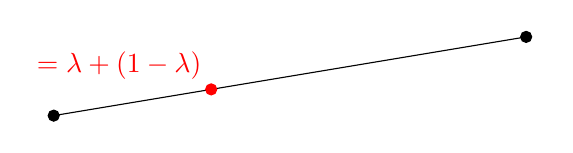
\begin{tikzpicture}

% Definisikan titik-titik
\coordinate (x) at (0,0);
\coordinate (y) at (6,1);
\coordinate (z) at (2/3*0 + 1/3*6, 2/3*0 + 1/3*1);

% Gambar ruas garis antara x dan y
\draw (x) -- (y);

% Tandai titik-titik dengan noktah dan label
\filldraw [black] (x) circle (2pt) node[anchor=east] {$\x$};
\filldraw [black] (y) circle (2pt) node[anchor=west] {$\y$};
\filldraw [red] (z) circle (2pt) node[anchor=south east] {$\z = \lambda \x + (1-\lambda)\y$};

\end{tikzpicture}
\end{center}
\caption{Kombinasi konveks titik $\x$ dan $\y$ diberikan oleh $\z = \lambda \x + (1-\lambda)\y$ untuk setiap $\lambda \in [0,1]$. Di sini kita memperagakannya dengan $\lambda = 2/3$.}
\end{figure}

\begin{definition}{Himpunan Konveks}
Himpunan $C$ bersifat konveks jika memuat semua kombinasi konveks dari titik-titik dalam $C$. Artinya, untuk setiap $\x,\y \in C$, berlaku $ \lambda \x + (1-\lambda) \y \in C$ untuk semua $\lambda \in [0,1]$.
\end{definition}

\begin{figure}[h!]
  \begin{subfigure}[b]{0.45\textwidth}
    \centering
    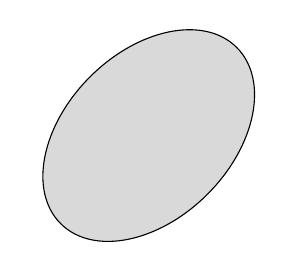
\begin{tikzpicture}
        \draw[rotate=-45,fill=gray!30, thin] (0,0) ellipse (30pt and 45pt);
    \end{tikzpicture}
    \caption{Himpunan Konveks}
    \label{fig:convex-set-example}
  \end{subfigure}
  \begin{subfigure}[b]{0.45\textwidth}
    \centering
    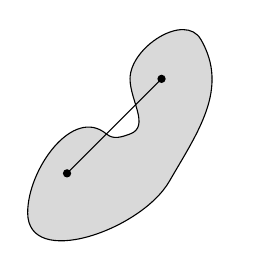
\begin{tikzpicture}
        \useasboundingbox (-1,-1.35) rectangle (1.5,1.35); 
        \draw[fill=gray!30, thin] (0,0) to [out=140,in=90] (-1,-1)
        to [out=-90,in=240] (0.8,-0.6)
        to [out=60,in=-60] (1.2,1.2)
        to [out=120,in=90] (0.3,0.7)
        to [out=-90,in=20] (0.3,0)
        to [out=200,in=-40] (0,0);
        \draw[thin] (-0.5,-0.5) -- (0.7,0.7);
        \fill (-0.5,-0.5) circle[radius=1.5pt];
        \fill (0.7,0.7) circle[radius=1.5pt];
    \end{tikzpicture}
    \caption{Himpunan Tak Konveks}
    \label{fig:nonconvex-set-example}
  \end{subfigure}
\caption{Himpunan konveks dan himpunan tak konveks.}\label{fig:convex-nonconvex-examples}% fig-num-auto
\end{figure}

Beberapa contoh himpunan konveks adalah:
\begin{enumerate}
    \item \emph{Hiperbidang}  $H = \{\x \in \R^n : \a^\top \x = b\}$
    \item \emph{Setengah ruang}   $H = \{ \x \in \R^n : \a^\top \x \leq b\}$
    \item \emph{Polihedron}  $P = \{\x \in \R^n : A\x \leq \b\}$
    \item \emph{Bola} $B = \{ \x \in \R^n : \sum_{i=1}^n x_i^2 \leq 1\}$
    \item \emph{Kerucut orde dua} $S = \{ (\x,t) \in \R^n \times \R : \|\x\| \leq t \}$, yaitu $\sum_{i=1}^n x_i^2 \leq t^2$ dengan $t \geq 0$
\end{enumerate}

\begin{figure}[h!]
\centering
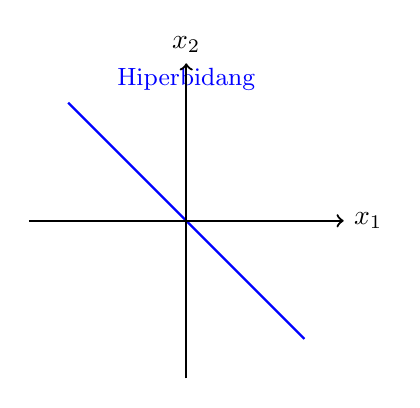
\begin{tikzpicture}[scale=1]
    % Hiperbidang
    \draw[blue, thick] (-1.5,1.5) -- (1.5,-1.5);
    \node[blue] at (0,1.8) {\small Hiperbidang};
    % Sumbu
   \draw[->,thick] (-2,0) -- (2,0) node[right] {$x_1$};
    \draw[->,thick] (0,-2) -- (0,2) node[above] {$x_2$};
\end{tikzpicture}
\hfill
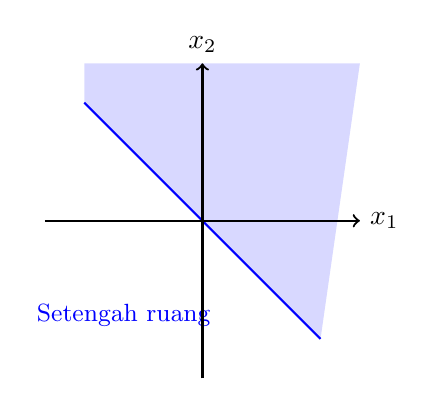
\begin{tikzpicture}[scale=1]
    % Setengah ruang
    \fill[blue!30,opacity=0.5] (-1.5,1.5) -- (1.5,-1.5) -- (2,2) -- (-1.5,2) -- cycle;
    \draw[blue, thick] (-1.5,1.5) -- (1.5,-1.5);
    \node[blue] at (-1,-1.2) {\small Setengah ruang};
    % Sumbu
    \draw[->,thick] (-2,0) -- (2,0) node[right] {$x_1$};
    \draw[->,thick] (0,-2) -- (0,2) node[above] {$x_2$};
\end{tikzpicture}
\hfill
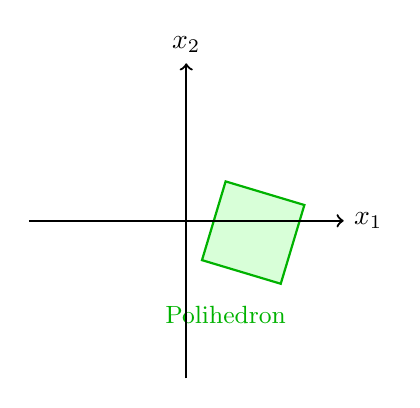
\begin{tikzpicture}[scale=1]
    % Polihedron
    \fill[green!30,opacity=0.5] (0.5,0.5) -- (1.5,0.2) -- (1.2,-0.8) -- (0.2,-0.5) -- cycle;
    \draw[green!70!black, thick] (0.5,0.5) -- (1.5,0.2) -- (1.2,-0.8) -- (0.2,-0.5) -- cycle;
    \node[green!70!black] at (0.5,-1.2) {\small Polihedron};
    % Sumbu
    \draw[->,thick] (-2,0) -- (2,0) node[right] {$x_1$};
    \draw[->,thick] (0,-2) -- (0,2) node[above] {$x_2$};
\end{tikzpicture}

\par\vspace{1.2em}

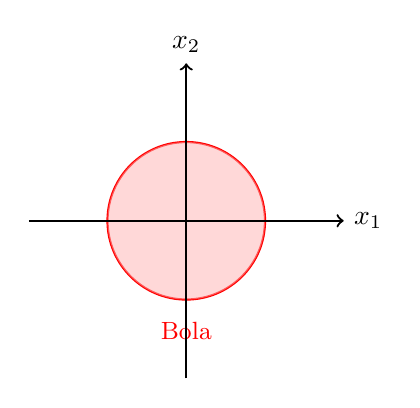
\begin{tikzpicture}[scale=1]
    % Bola
    \draw[red, thick] (0,0) circle (1cm);
    \fill[red!30,opacity=0.5] (0,0) circle (1cm);
    \node[red] at (0,-1.4) {\small Bola};
    % Sumbu
    \draw[->,thick] (-2,0) -- (2,0) node[right] {$x_1$};
    \draw[->,thick] (0,-2) -- (0,2) node[above] {$x_2$};
\end{tikzpicture}
\hspace{2em}
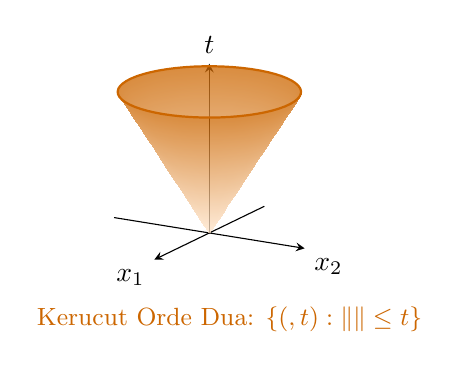
\begin{tikzpicture}
% Kerucut orde dua dalam R^3: ||(x1,x2)|| <= t
% Kompatibilitas ditetapkan secara lokal: preambul buku tidak memuat \pgfplotsset{compat=...},
% dan penempatan label sumbu pada kompatibilitas lama menyebarkan t/x2 ke seluruh halaman.
\pgfplotsset{compat=1.16}
\begin{axis}[
    width=5.4cm, height=4.8cm,
    view={120}{20},
    axis lines=center,
    ticks=none,
    xlabel={$x_1$}, ylabel={$x_2$}, zlabel={$t$},
    xlabel style={anchor=north east},
    ylabel style={anchor=north west},
    zlabel style={anchor=south},
    zmin=0, zmax=1.2,
    xmin=-1.2, xmax=1.2, ymin=-1.2, ymax=1.2,
    clip=false]
  % permukaan sisi kerucut t = ||(x1,x2)||
  \addplot3[surf, shader=interp,
      colormap={soc}{color=(orange!20) color=(orange!80!black)},
      opacity=0.75, domain=0:1, y domain=0:360,
      samples=14, samples y=40, z buffer=sort]
      ({x*cos(y)}, {x*sin(y)}, {x});
  % tepian kerucut pada t = 1
  \addplot3[orange!80!black, thick, domain=0:360, samples=60]
      ({cos(x)}, {sin(x)}, {1});
\end{axis}
\node[orange!80!black, below=1pt] at (current bounding box.south)
    {\small Kerucut Orde Dua: $\{(\x, t) : \|\x\| \leq t\}$};
\end{tikzpicture}

\caption{Contoh himpunan konveks: hiperbidang, setengah ruang, polihedron, bola, dan kerucut orde dua.}\label{fig:convex-set-examples}% fig-num-auto
\end{figure}

\begin{lemma}{Irisan Himpunan Konveks Bersifat Konveks}
Misalkan $C_1$ dan $C_2$ adalah himpunan konveks. Maka irisan $C_1 \cap C_2$ bersifat konveks.  
Secara khusus, 
$$C_1 \cap C_2 := \{ \x :  \x \in C_1 \ \text{ dan } \x \in C_2\}.
$$
\end{lemma}

\begin{figure}[h]
\begin{center}
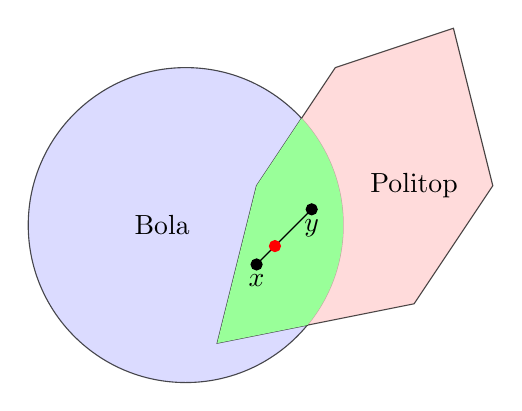
\begin{tikzpicture}

% Gambar lingkaran (bola dalam 2D) sedikit ke kiri
\filldraw[blue!20, opacity=0.7, draw = black] (0.1,1.5) circle (2cm);

% Gambar politop 6 titik sudut sedikit ke kanan
\filldraw[red!20, opacity=0.7, draw = black] (0.5,0) -- (3,0.5) -- (4,2) -- (3.5,4) -- (2,3.5) -- (1,2) -- cycle;

% Arsir irisannya
\begin{scope}
  \clip (0.1,1.5) circle (2cm);
  \fill[green!40] (0.5,0) -- (3,0.5) -- (4,2) -- (3.5,4) -- (2,3.5) -- (1,2) -- cycle;
\end{scope}

% Beri label pada lingkaran dan politop
\node at (-0.2,1.5) {Bola};
\node at (3,2) {Politop};

% Definisikan titik-titik
\coordinate (x) at (1,1);
\coordinate (y) at (1.7,1.7);
\coordinate (z) at (2/3*1 + 1/3*1.7, 2/3*1 + 1/3*1.7);

% Gambar ruas garis antara x dan y
\draw (x) -- (y);

% Tandai titik-titik dengan noktah dan label
\filldraw [black] (x) circle (2pt) node[anchor=north] {$x$};
\filldraw [black] (y) circle (2pt) node[anchor=north] {$y$};
\filldraw [red] (z) circle (2pt) node[anchor=south east] {};%$z = \lambda x + (1-\lambda)y$};
\end{tikzpicture}\vspace{1cm}
\end{center}
\caption{Irisan hijau dari himpunan konveks berupa bola dan politop juga bersifat konveks. Hal ini dapat dilihat dengan memilih sembarang titik $x,y \in \text{Bola} \cap \text{Politop}$. Karena Bola bersifat konveks, ruas garis antara $x$ dan $y$ seluruhnya termuat dalam Bola. Demikian pula, ruas garis tersebut seluruhnya termuat dalam Politop. Jadi, ruas garis itu juga termuat dalam irisannya. Dengan penalaran ini, kita mengetahui bahwa irisan tersebut juga bersifat konveks.} 
\end{figure}

%
\begin{theorem}{Konveksitas Polihedron}
\label{thm:polyhedra_convex}
Sebuah polihedron \( P = \{\mathbf{x} \in \mathbb{R}^n : A\mathbf{x} \leq \mathbf{b}\} \), yakni irisan sejumlah berhingga setengah ruang, merupakan himpunan konveks.
\end{theorem}
%
\begin{proof}
Secara intuitif, konveksitas berarti ruas garis antara dua titik mana pun dalam himpunan tetap berada di dalam himpunan tersebut. Untuk polihedron yang didefinisikan oleh pertidaksamaan linier, sifat ini langsung mengikuti linearitas pertidaksamaan tersebut, seperti yang sekarang kita tunjukkan.

Misalkan \( P \) adalah polihedron dalam \(\mathbb{R}^n\) yang didefinisikan oleh irisan sejumlah berhingga setengah ruang:
\[
P = \{\mathbf{x} \in \mathbb{R}^n : A\mathbf{x} \leq \mathbf{b}\},
\]
dengan \(A\) sebagai matriks \(m \times n\), \(\mathbf{x} \in \mathbb{R}^n\) sebagai vektor variabel, dan \(\mathbf{b} \in \mathbb{R}^m\) sebagai vektor konstan.

Untuk membuktikan bahwa \(P\) bersifat konveks, kita harus menunjukkan bahwa untuk setiap dua titik \(\mathbf{x}_1, \mathbf{x}_2 \in P\) dan setiap \(\lambda \in [0, 1]\), kombinasi konveks
\[
\mathbf{x}_\lambda = \lambda \mathbf{x}_1 + (1 - \lambda) \mathbf{x}_2
\]
juga terletak dalam \(P\). Dengan kata lain, kita perlu memverifikasi bahwa \(\mathbf{x}_\lambda\) memenuhi setiap kendala yang mendefinisikan \(P\), yaitu \(A\mathbf{x}_\lambda \leq \mathbf{b}\).

Karena \(\mathbf{x}_1, \mathbf{x}_2 \in P\), keduanya memenuhi pertidaksamaan yang mendefinisikan himpunan tersebut:
\[
A\mathbf{x}_1 \leq \mathbf{b} \quad \text{dan} \quad A\mathbf{x}_2 \leq \mathbf{b}.
\]
Berdasarkan linearitas perkalian matriks, kita dapat mendistribusikan \(A\) pada kombinasi konveks:
\[
A\mathbf{x}_\lambda = A(\lambda \mathbf{x}_1 + (1 - \lambda) \mathbf{x}_2) = \lambda A\mathbf{x}_1 + (1 - \lambda) A\mathbf{x}_2.
\]
Karena \(\lambda \geq 0\) dan \(1-\lambda \geq 0\), mengalikan pertidaksamaan \(A\mathbf{x}_1 \leq \mathbf{b}\) dan \(A\mathbf{x}_2 \leq \mathbf{b}\) dengan skalar-skalar tak negatif tersebut mempertahankan arahnya. Penjumlahan kedua pertidaksamaan yang telah diskalakan menghasilkan
\[
\lambda A\mathbf{x}_1 + (1 - \lambda) A\mathbf{x}_2 \leq \lambda \mathbf{b} + (1 - \lambda) \mathbf{b} = \mathbf{b}.
\]
Dengan menggabungkan kedua baris yang ditampilkan, kita menyimpulkan bahwa \(A\mathbf{x}_\lambda \leq \mathbf{b}\), sehingga \(\mathbf{x}_\lambda \in P\).

Karena \(\mathbf{x}_1\), \(\mathbf{x}_2\), dan \(\lambda\) dipilih secara sembarang, setiap kombinasi konveks titik-titik dalam \(P\) tetap berada dalam \(P\). Jadi, \(P\) bersifat konveks.
\end{proof}
%
%

\textbf{Titik Ekstrem:}  
Titik ekstrem suatu himpunan polihedral \(C\) adalah titik yang tidak dapat ditulis sebagai kombinasi konveks dari titik-titik lain dalam \(C\). Solusi program linier sering terjadi pada titik ekstrem, sebagaimana dijamin oleh teorema-teorema dasar program linier.

\begin{lemma}{Nilai Objektif pada Ruas Garis}
\label{lemma:objective_bound}
Diberikan dua titik \(\mathbf{x}, \mathbf{y} \in \mathbb{R}^n\), nilai fungsi linier pada setiap titik di ruas garis antara \(\mathbf{x}\) dan \(\mathbf{y}\) dibatasi dari atas oleh nilai maksimum evaluasi pada \(\mathbf{x}\) dan \(\mathbf{y}\). Secara formal, untuk setiap \(\mathbf{c} \in \mathbb{R}^n\),
\[
\min\{\mathbf{c}^\top \mathbf{x}, \mathbf{c}^\top \mathbf{y}\} \leq \mathbf{c}^\top \mathbf{z} \leq \max\{\mathbf{c}^\top \mathbf{x}, \mathbf{c}^\top \mathbf{y}\},
\]
dengan \(\mathbf{z} = \lambda \mathbf{x} + (1-\lambda) \mathbf{y}\) untuk suatu $\lambda \in (0,1)$.

Kedua pertidaksamaan ini dapat sama-sama ketat atau sama-sama berlaku sebagai persamaan.
\end{lemma}

\begin{proof}
Dengan menguraikan $\mathbf{c}^\top \mathbf{z}$ berdasarkan definisinya,
\begin{align*}
\mathbf{c}^\top \mathbf{z}  &= \mathbf{c}^\top (\lambda \mathbf{x} + (1-\lambda) \mathbf{y}) & \text{Ganti rumus $\mathbf{z}$}\\
& =  \mathbf{c}^\top \lambda\mathbf{x} +  \mathbf{c}^\top (1-\lambda)\mathbf{y} & \text{ gunakan sifat distributif}\\
& = \lambda \mathbf{c}^\top \mathbf{x} + (1-\lambda) \mathbf{c}^\top\mathbf{y} & \text{ gunakan linearitas}
\end{align*}

Persamaan ini menyatakan \(\mathbf{c}^\top \mathbf{z}\) sebagai kombinasi konveks dari \(\mathbf{c}^\top \mathbf{x}\) dan \(\mathbf{c}^\top \mathbf{y}\). Karena \(\lambda \in [0, 1]\), kita mengetahui bahwa \(\lambda \geq 0\) dan \(1-\lambda \geq 0\), sehingga kombinasinya bersifat konveks.

\begin{center}
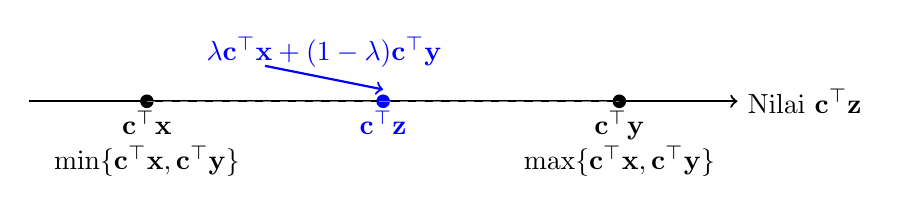
\begin{tikzpicture}[scale=1.5]
    % Gambar garis 1D
    \draw[thick, ->] (0, 0) -- (6, 0) node[right] {Nilai $\mathbf{c}^\top \mathbf{z}$};

    % Titik-titik untuk c^T x, c^T y, dan c^T z
    \filldraw[black] (1, 0) circle (1.5pt) node[below] {$\mathbf{c}^\top \mathbf{x}$};
    \filldraw[black] (5, 0) circle (1.5pt) node[below] {$\mathbf{c}^\top \mathbf{y}$};
    
    % Titik untuk c^T z (di suatu tempat di antaranya)
    \filldraw[blue] (3, 0) circle (1.5pt) node[below] {$\mathbf{c}^\top \mathbf{z}$};

    % Anotasikan kombinasi konveks
    \draw[dashed, gray] (1, 0) -- (3, 0);
    \draw[dashed, gray] (3, 0) -- (5, 0);

    % Tambahkan batas minimum dan maksimum
    \node[below] at (1, -0.3) {$\min\{\mathbf{c}^\top \mathbf{x}, \mathbf{c}^\top \mathbf{y}\}$};
    \node[below] at (5, -0.3) {$\max\{\mathbf{c}^\top \mathbf{x}, \mathbf{c}^\top \mathbf{y}\}$};

    % Tambahkan panah penjelas untuk kombinasi konveks
    \draw[->, thick, blue] (2, 0.3) -- (3, 0.1) node[midway, above] {$\lambda \mathbf{c}^\top \mathbf{x} + (1-\lambda) \mathbf{c}^\top \mathbf{y}$};

\end{tikzpicture}\par\captionof{figure}{Garis bilangan yang menunjukkan bahwa nilai objektif pada z terletak di antara nilai objektif pada x dan y.}\label{fig:formalize-LP-tikz10}% fig-num-auto

\end{center}

Berdasarkan sifat kombinasi konveks, nilai \(\mathbf{c}^\top \mathbf{z}\) terletak di antara \(\mathbf{c}^\top \mathbf{x}\) dan \(\mathbf{c}^\top \mathbf{y}\). Secara formal:
\[
\min\{\mathbf{c}^\top \mathbf{x}, \mathbf{c}^\top \mathbf{y}\} \leq \mathbf{c}^\top \mathbf{z} \leq \max\{\mathbf{c}^\top \mathbf{x}, \mathbf{c}^\top \mathbf{y}\}.
\]

Jadi, nilai \(\mathbf{c}^\top \mathbf{z}\) dibatasi dari atas oleh \(\max\{\mathbf{c}^\top \mathbf{x}, \mathbf{c}^\top \mathbf{y}\}\), sebagaimana yang harus dibuktikan.
\end{proof}

\begin{theorem}{Solusi Optimal pada Titik Ekstrem}
\label{thm:extreme_point_optimum}
Misalkan \(C \subseteq \mathbb{R}^n\) adalah himpunan terbatas, tertutup, dan konveks. Misalkan objektifnya adalah memaksimumkan \(\mathbf{c}^\top \mathbf{x}\) atas \(C\). Maka terdapat solusi optimal \(\mathbf{x}^* \in C\) sedemikian sehingga \(\mathbf{x}^*\) merupakan titik ekstrem \(C\).
\end{theorem}

\begin{proof}
Karena \(C\) terbatas dan tertutup, himpunan tersebut kompak dalam \(\mathbb{R}^n\). Fungsi linier \(\mathbf{c}^\top \mathbf{x}\) kontinu, dan berdasarkan Teorema Nilai Ekstrem, fungsi tersebut mencapai nilai maksimumnya pada himpunan kompak \(C\). Misalkan \(\mathbf{x}^* \in C\) sedemikian sehingga:
\[
\mathbf{c}^\top \mathbf{x}^* = \max \{ \mathbf{c}^\top \mathbf{x} : {\mathbf{x} \in C} \}
\]

Misalkan \(\mathbf{x}^*\) bukan titik ekstrem \(C\). Maka \(\mathbf{x}^*\) dapat dinyatakan sebagai kombinasi konveks dari dua titik berbeda \(\mathbf{x}, \mathbf{y} \in C\):
\[
\mathbf{x}^* = \lambda \mathbf{x} + (1-\lambda) \mathbf{y}, \quad \text{dengan } \lambda \in (0, 1).
\]

Berdasarkan Lema~\ref{lemma:objective_bound}, nilai \(\mathbf{c}^\top \mathbf{x}^*\) memenuhi:
\[
\min\{\mathbf{c}^\top \mathbf{x}, \mathbf{c}^\top \mathbf{y}\} \leq \mathbf{c}^\top \mathbf{x}^* \leq \max\{\mathbf{c}^\top \mathbf{x}, \mathbf{c}^\top \mathbf{y}\}.
\]

Karena \(\mathbf{x}^*\) memaksimumkan \(\mathbf{c}^\top \mathbf{x}\) atas \(C\), harus berlaku \(\mathbf{c}^\top \mathbf{x} = \mathbf{c}^\top \mathbf{x}^*\) dan \(\mathbf{c}^\top \mathbf{y} = \mathbf{c}^\top \mathbf{x}^*\). Jadi, \(\mathbf{x}\) dan \(\mathbf{y}\) juga memaksimumkan \(\mathbf{c}^\top \mathbf{x}\) atas \(C\).

Jika \(\mathbf{x}^*\) bukan titik ekstrem, kita dapat mengulangi argumen ini untuk \(\mathbf{x}\) dan \(\mathbf{y}\), dengan menyatakannya sebagai kombinasi konveks dari titik-titik lain dalam \(C\). Jika \(C\) merupakan polihedron, proses ini harus berhenti setelah sejumlah langkah berhingga karena setiap langkah berpindah ke muka yang dimensinya lebih kecil secara ketat dan sebuah polihedron hanya memiliki sejumlah muka berhingga; pada saat itu kita mencapai titik ekstrem yang memaksimumkan \(\mathbf{c}^\top \mathbf{x}\). (Untuk himpunan konveks kompak umum, penghentian memerlukan argumen yang lebih saksama, misalnya induksi pada dimensi \(C\); perinciannya tidak diberikan di sini.)

Jadi, terdapat solusi optimal pada sebuah titik ekstrem \(C\).
\end{proof}

\begin{theorem}{Titik Ekstrem dan Titik Sudut Polihedron}
Misalkan \( P \subseteq \mathbb{R}^n \) adalah sebuah polihedron. Maka titik \( \mathbf{v} \in P \) merupakan titik ekstrem jika dan hanya jika \( \mathbf{v} \) merupakan titik sudut \( P \).
\end{theorem}

\begin{proof}
\textbf{(Jika \( \mathbf{v} \) bukan titik sudut, maka ia bukan titik ekstrem):}

Misalkan \( \mathbf{v} \in P \) bukan titik sudut. Menurut definisi, ini berarti \( \mathbf{v} \) bukan solusi tunggal bagi subhimpunan mana pun yang terdiri atas \( n \) kendala bebas linier yang aktif pada \( \mathbf{v} \). Misalkan \( A' \mathbf{x} = \mathbf{b}' \) menyatakan kendala aktif pada \( \mathbf{v} \), dengan \( A' \in \mathbb{R}^{m' \times n} \) (\( m' \leq n \)) sebagai matriks kendala aktif, dan anggap baris-baris \( A' \) bebas linier. Karena \( \mathbf{v} \) bukan titik sudut, ruang nol \( A' \), yang dinyatakan dengan \( \mathcal{N}(A') \), tidak trivial. Artinya, terdapat arah tak nol \( \mathbf{d} \in \mathbb{R}^n \) sedemikian sehingga:
\[
A' \mathbf{d} = \mathbf{0}.
\]

Perhatikan gangguan pada \( \mathbf{v} \) ke arah \( \mathbf{v} + \epsilon \mathbf{d} \) dan \( \mathbf{v} - \epsilon \mathbf{d} \), untuk suatu \( \epsilon > 0 \) yang kecil. Karena \( \mathbf{d} \in \mathcal{N}(A') \), titik-titik yang diganggu memenuhi kendala aktif:
\[
A' (\mathbf{v} + \epsilon \mathbf{d}) = A' \mathbf{v} + \epsilon A' \mathbf{d} = \mathbf{b}'.
\]
Demikian pula, \( A' (\mathbf{v} - \epsilon \mathbf{d}) = \mathbf{b}' \).

Untuk \( \epsilon > 0 \) yang cukup kecil, titik-titik yang diganggu juga memenuhi semua kendala lain yang mendefinisikan \( P \). Hal ini karena \( P \) merupakan polihedron dan kendala-kendalanya adalah pertidaksamaan linier kontinu yang tetap terpenuhi di bawah gangguan kecil terhadap \( \mathbf{v} \).

Sekarang kita menyatakan \( \mathbf{v} \) sebagai kombinasi konveks ketat dari \( \mathbf{v} + \epsilon \mathbf{d} \) dan \( \mathbf{v} - \epsilon \mathbf{d} \):
\[
\mathbf{v} = \frac{1}{2} (\mathbf{v} + \epsilon \mathbf{d}) + \frac{1}{2} (\mathbf{v} - \epsilon \mathbf{d}).
\]
Karena \( \mathbf{v} + \epsilon \mathbf{d} \neq \mathbf{v} \) dan \( \mathbf{v} - \epsilon \mathbf{d} \neq \mathbf{v} \), serta kedua titik tersebut berada dalam \( P \), hal ini menunjukkan bahwa \( \mathbf{v} \) bukan titik ekstrem \( P \).

\begin{center}
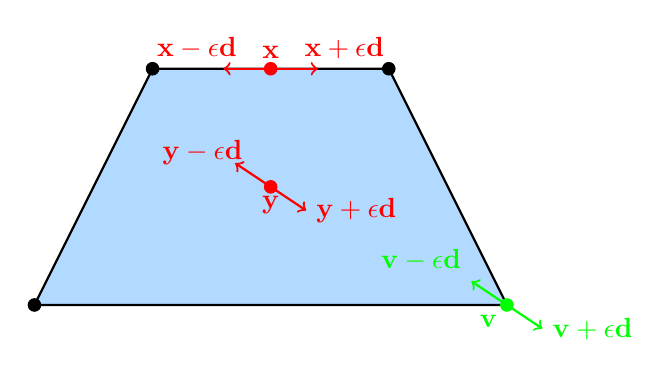
\begin{tikzpicture}[scale=1.5]
    % Gambar politop
    \fill[blue!50!cyan,opacity=0.3] (0,0) -- (1,2) -- (3,2) -- (4,0) -- cycle;

    % Gambar sisi-sisi politop
    \draw[thick] (0,0) -- (1,2) -- (3,2) -- (4,0) -- cycle;

    % Beri label titik-titik sudut
    \filldraw[black] (0,0) circle (1.5pt);
    \filldraw[black] (1,2) circle (1.5pt);
    \filldraw[black] (3,2) circle (1.5pt);
    \filldraw[green] (4,0) circle (1.5pt) node[below left] {$\mathbf{v}$};

    % Tandai titik x pada sisi
    \filldraw[red] (2,2) circle (1.5pt) node[above] {$\mathbf{x}$};

    % Gambar arah gangguan pada sisi
    \draw[->, thick, red] (2,2) -- (2.4,2) node[midway, above right] {$\mathbf{x} + \epsilon \mathbf{d}$};
    \draw[->, thick, red] (2,2) -- (1.6,2) node[midway, above left] {$\mathbf{x} - \epsilon \mathbf{d}$};

    % Tandai titik lain di dalam politop
    \filldraw[red] (2,1) circle (1.5pt) node[below] {$\mathbf{y}$};

    % Gambar arah gangguan di dalam politop
    \draw[->, thick, red] (2,1) -- (2.3,0.8) node[right] {$\mathbf{y} + \epsilon \mathbf{d}$};
    \draw[->, thick, red] (2,1) -- (1.7,1.2) node[midway, above left] {$\mathbf{y} - \epsilon \mathbf{d}$};

    % Gambar arah gangguan bagi titik sudut hijau
    \draw[->, thick, green] (4,0) -- (4.3,-0.2) node[right] {$\mathbf{v} + \epsilon \mathbf{d}$};
    \draw[->, thick, green] (4,0) -- (3.7,0.2) node[above left] {$\mathbf{v} - \epsilon \mathbf{d}$};

\end{tikzpicture}\par\captionof{figure}{Gambar dua dimensi politop segi empat dengan titik sudut (0,0), (1,2), (3,2), (4,0).}\label{fig:formalize-LP-tikz11}% fig-num-auto

\end{center}

\textbf{(Jika \(\mathbf{v}\) merupakan titik sudut, maka ia merupakan titik ekstrem):}

Anggap \( \mathbf{v} \in P \) merupakan titik sudut. Menurut definisi, terdapat sebuah subhimpunan kendala, misalnya \( A'\mathbf{x} = \mathbf{b}' \), dengan \( A' \in \mathbb{R}^{n \times n} \), sedemikian sehingga \( \mathbf{v} \) merupakan solusi tunggal sistem ini.

Untuk memperoleh pertentangan, misalkan \( \mathbf{v} \) bukan titik ekstrem. Maka \( \mathbf{v} \) dapat dinyatakan sebagai:
\[
\mathbf{v} = \lambda \mathbf{x}_1 + (1 - \lambda) \mathbf{x}_2, \quad \mathbf{x}_1, \mathbf{x}_2 \in P, \, \lambda \in (0, 1),
\]
dengan \( \mathbf{x}_1 \neq \mathbf{v} \) dan \( \mathbf{x}_2 \neq \mathbf{v} \).

Kita menyatakan bahwa \( \mathbf{x}_1 \) dan \( \mathbf{x}_2 \) harus memenuhi \( A'\mathbf{x} = \mathbf{b}' \). Untuk melihatnya,
misalkan $\mathbf{a}$ adalah sebuah baris $A'$ dan $b$ adalah nilai ruas kanan yang bersesuaian dalam $\mathbf{b}'$.
Berdasarkan Lema~\ref{lemma:objective_bound}, nilai \( \mathbf{a}^\top \mathbf{v} \) memenuhi:
\[
\min\{\mathbf{a}^\top\mathbf{x}_1, \mathbf{a}^\top\mathbf{x}_2\} \leq \mathbf{a}^\top\mathbf{v} \leq \max\{\mathbf{a}^\top\mathbf{x}_1, \mathbf{a}^\top\mathbf{x}_2\}.
\]
Karena \( \mathbf{v} \) memenuhi \( \mathbf{a}^\top\mathbf{v} = b\), hal ini menyiratkan:
\[
\mathbf{a}^\top\mathbf{v} = \lambda \mathbf{a}^\top\mathbf{x}_1 + (1-\lambda) \mathbf{a}^\top\mathbf{x}_2 = b.
\]

Jika \( \mathbf{a}^\top\mathbf{x}_1 \neq b \) atau \( \mathbf{a}^\top\mathbf{x}_2 \neq b\), persamaan di atas tidak mungkin berlaku. Jadi, \( \mathbf{x}_1 \) dan \( \mathbf{x}_2 \) harus memenuhi \( \mathbf{a}^\top\mathbf{x} = b \).

Karena \( \mathbf{v} \) memenuhi \( A'\mathbf{x} = \mathbf{b}' \), \( \mathbf{x}_1 \) dan \( \mathbf{x}_2 \) juga harus memenuhi \( A'\mathbf{x} = \mathbf{b}' \), sebab \( A'\mathbf{x} = \mathbf{b}' \) mendefinisikan subruang afin. Namun, hal ini bertentangan dengan asumsi bahwa \( \mathbf{v} \) merupakan solusi tunggal \( A'\mathbf{x} = \mathbf{b}' \).

Oleh karena itu, \( \mathbf{v} \) tidak dapat dinyatakan sebagai kombinasi konveks ketat dari titik-titik berbeda dalam \( P \), dan \( \mathbf{v} \) merupakan titik ekstrem.

\textbf{Kesimpulan:} Titik \( \mathbf{v} \in P \) merupakan titik ekstrem jika dan hanya jika merupakan titik sudut \( P \).
\end{proof}

\subsection{Himpunan Tak Berbatas dan Sinar}

\textbf{Sinar dan Arah:}  
Sinar dalam \(\mathbb{R}^n\) adalah himpunan titik:
\[
\{\mathbf{x} : \mathbf{x} = \mathbf{\bar x} + \lambda \mathbf{d}, \, \lambda \geq 0\},
\]
dengan \(\mathbf{\bar x}\) sebagai titik awal dan \(\mathbf{d}\) sebagai arah. Sinar menggambarkan daerah layak tak berbatas dalam model program linier.

\textbf{Arah Ekstrem:}  
Arah ekstrem adalah arah yang tidak dapat ditulis sebagai kombinasi positif dari arah-arah lain. Dalam program linier, arah ekstrem membantu mencirikan solusi tak berbatas.

\medskip
Dengan konsep-konsep ini, kita dapat menyatakan hasil struktural: setiap titik polihedron \( P \) dapat dibentuk dari titik ekstrem dan arah ekstrem \( P \).

\begin{theorem}{Teorema Representasi}
\label{thm:representation}
 Misalkan \( P \subseteq \mathbb{R}^n \) adalah polihedron tak kosong, misalkan $\mathbf{x}^1, \mathbf{x}^2,\cdots \mathbf{x}^k$ adalah himpunan titik ekstrem $P$, dan jika $P$ tak berbatas, misalkan $\mathbf{d}^1, \mathbf{d}^2,\cdots \mathbf{d}^l$ adalah himpunan arah ekstremnya. Maka setiap $\mathbf{x} \in P$ sama dengan kombinasi konveks titik-titik ekstrem dan kombinasi linier tak negatif arah-arah ekstrem: $\mathbf{x} = \sum_{j=1}^k \lambda_j \mathbf{x}^j + \sum_{j=1}^l \mu_j \mathbf{d}^j$, dengan $\sum_{j=1}^k \lambda_j = 1$, $\lambda_j \ge 0,~\forall  j=1,2,\cdots,k$, dan $\mu_j \ge 0,~\forall j=1,2,\cdots,l$.
 \end{theorem}

Sebagai ilustrasi, perhatikan program linier di bawah ini. Daerah layaknya \( P \) digambar di sebelah kanan (pada bidang \((x_1,x_2)\), dengan variabel kelonggaran \(s_1, s_2, s_3\) dieliminasi). Daerah layak ini tak berbatas dan memanjang tanpa batas ke kanan atas. Karena itulah teorema harus mengizinkan arah ekstrem. Titik-titik ekstremnya adalah \((0,0)\), \((0,1)\), dan \((2,3)\), yang ditandai dalam gambar.

 \begin{minipage}[t][][b]{.4\linewidth}
\begin{align*}
\max \quad & z = -5x_1 - x_2  \\
\text{dengan syarat} \quad & x_1 - 4x_2 +s_1 = 0  \\
& -x_1 + x_2 + s_2 = 1 \\
& -x_1 + 2x_2 +s_3 = 4 \\
& x_1, x_2, s_1, s_2, s_3 \ge 0.
\end{align*}
\end{minipage}%
\begin{minipage}[t][][b]{.6\linewidth}
\begin{center}  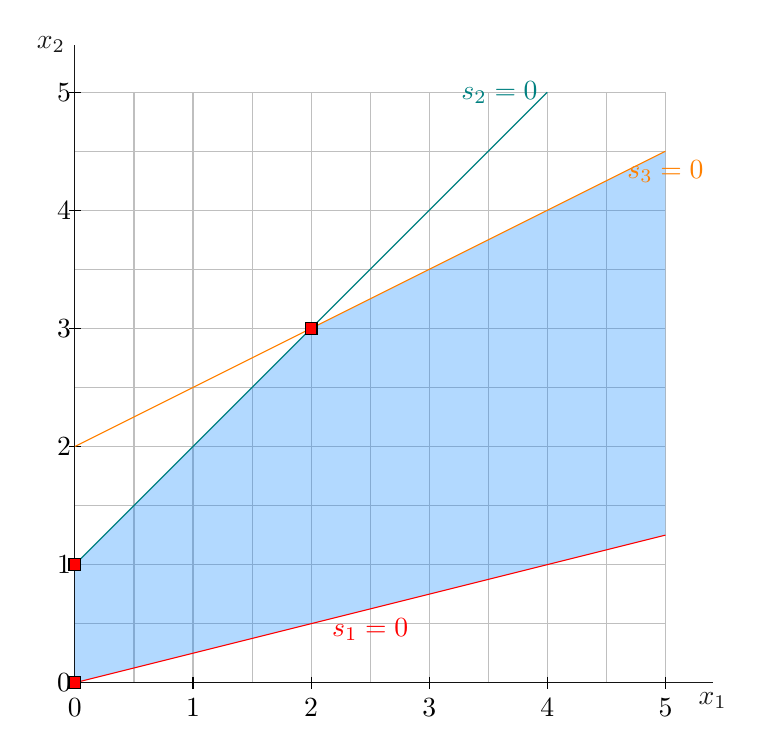
\begin{tikzpicture} [scale=1.5]
    \draw[gray!50, thin, step=.5] (0,0) grid (5,5);
    \draw[opacity=0.9] (0,0) -- (5.4,0) node[below] {$x_1$};
    \draw[opacity=0.9] (0,0) -- (0,5.4) node[left] {$x_2$}; % pilihan \draw[very thick,->]

    \foreach \x in {0,...,5} \draw (\x,0.05) -- (\x,-0.05) node[below] {\x};
    \foreach \y in {0,...,5} \draw (-0.05,\y) -- (0.05,\y) node[left] {\y};

    \fill[blue!50!cyan,opacity=0.3] (0,0) -- (0,1) -- (2,3) -- (5,4.5) --(5,1.25)-- cycle;

    \draw [red](0,0) -- node[below] {$s_1=0$} (5, 1.25);
    \draw [teal] (0,1)  --  (4,5) node[left, sloped] {$s_2=0$};
    \draw [orange](0,2) --  (5,4.5) node[below, sloped] {$s_3=0$}; %node[above right ,sloped] 
    \node[fill=blue,circle,inner sep=0.05cm] at (0,0) {};
\node[fill=blue,circle,inner sep=0.05cm] at (0,1) {};
\node[fill=blue,circle,inner sep=0.05cm] at (2,3) {};

\filldraw[fill=red] (-0.05,-0.05) rectangle (0.05,0.05);
\filldraw[fill=red] (-0.05,.95) rectangle (0.05,1.05);
\filldraw[fill=red] (1.95,2.95) rectangle (2.05,3.05);
\end{tikzpicture}\par\captionof{figure}{Daerah layak dengan garis s1=0, s2=0, dan s3=0 yang menandai tempat setiap variabel kelonggaran bernilai nol; solusi dasar ditandai oleh titik biru dan kotak merah.}\label{fig:formalize-LP-tikz12}% fig-num-auto
 \end{center} 
\end{minipage}

Sebagai penggunaan konkret teorema tersebut, kita menyatakan titik \((1/2, 1) \in P\) sebagai kombinasi konveks titik-titik ekstrem. Carilah $\lambda$ yang menyelesaikan sistem persamaan berikut, dengan syarat $\lambda_1 + \lambda_2 + \lambda_3 = 1$ dan $\lambda_1, \lambda_2, \lambda_3 \geq 0$:

$$\lambda_1 \left[
  \begin{array}{c}
  0 \\
  0 \\
  \end{array} \right]+
 \lambda_2 \left[
  \begin{array}{c}
  0 \\
  1 \\
  \end{array} \right] +
 \lambda_3 \left[
  \begin{array}{c}
  2 \\
  3 \\
  \end{array} \right]  =
 \left[
  \begin{array}{c}
  1/2 \\
  1 \\
  \end{array} \right]
$$

Salah satu solusinya adalah \(\lambda_1 = 1/2\), \(\lambda_2 = 1/4\), \(\lambda_3 = 1/4\): bobot-bobotnya tak negatif dan berjumlah \(1\), sehingga \((1/2,1)\) merupakan kombinasi konveks titik-titik ekstrem. Di sini tidak diperlukan arah ekstrem (semua \(\mu_j = 0\)); arah tersebut hanya diperlukan bagi titik-titik di luar selubung konveks titik-titik ekstrem, yaitu yang terletak lebih jauh dalam bagian \(P\) yang tak berbatas.

\section{Latihan}

\exgroup{Pemanasan}

\begin{ex}{Operasi Vektor}{}
\label{ex:vector-operations}
\stars{1}Misalkan \( \mathbf{v} = [3, -2, 4] \) dan \( \mathbf{u} = [-1, 0, 2] \). Hitung:
\begin{enumerate}
    \item \( \mathbf{v} + \mathbf{u} \)
    \item \( 2\mathbf{v} \)
    \item \( \mathbf{v} \cdot \mathbf{u} \)
\end{enumerate}
\exrefs{\S\ref{sec:math-preliminaries}}
\end{ex}

\begin{ex}{Kombinasi Linier dan Konveks}{}
\stars{1}Misalkan \( \mathbf{v}^1 = [1, 0] \), \( \mathbf{v}^2 = [0, 1] \), dan \( \mathbf{v}^3 = [1, 1] \).

\begin{enumerate}
    \item Manakah di antara vektor berikut yang merupakan kombinasi linier dari \( \mathbf{v}^1 \) dan \( \mathbf{v}^2 \)?  
    \begin{itemize}
        \item[(a)] \( [2, 3] \)  
        \item[(b)] \( [1, 1] \)  
        \item[(c)] \( [1, -1] \)
    \end{itemize}
    \item Apakah vektor \( [1/2, 1/2] \) merupakan kombinasi konveks dari sepasang vektor di atas?
\end{enumerate}
\exrefs{\S\ref{sec:math-preliminaries}, \S\ref{sec:convexity}}
\end{ex}

\begin{ex}{Kebebasan Linier dan Rank Matriks}{}
\stars{1}Perhatikan matriks \( A = \begin{bmatrix} 1 & 2 \\ 2 & 4 \end{bmatrix} \).
\begin{enumerate}
    \item Apakah baris-baris \( A \) bebas linier?
    \item Apakah kolom-kolomnya bebas linier?
    \item Berapakah \( \operatorname{rank}(A) \)?
\end{enumerate}
\exrefs{\S\ref{sec:math-preliminaries}}
\end{ex}

\begin{ex}{Konveks atau Tidak?}{}
\label{ex:convex-or-not}
\stars{1}Untuk setiap subhimpunan \( \mathbb{R}^2 \) berikut, tentukan apakah himpunan tersebut konveks, seperti pada Gambar~\ref{fig:convex-set-example} dan \ref{fig:nonconvex-set-example}. Jika himpunan tersebut tidak konveks, berikan dua titik dalam himpunan yang ruas penghubungnya keluar dari himpunan.
\begin{enumerate}
    \item Cakram \( D = \{ \mathbf{x} : x_1^2 + x_2^2 \leq 4 \} \).
    \item Cincin \( R = \{ \mathbf{x} : 1 \leq x_1^2 + x_2^2 \leq 4 \} \).
    \item Setengah ruang \( H = \{ \mathbf{x} : x_1 + 2x_2 \leq 3 \} \).
    \item Himpunan \( S = \{ \mathbf{x} : |x_1| \geq 1 \} \).
\end{enumerate}
\exrefs{\S\ref{sec:convexity}}
\end{ex}

\begin{ex}{Menulis Program Linier dalam Notasi Matriks}{}
\label{ex:lp-matrix-notation}
\stars{1}Perhatikan program linier
\begin{align*}
\max \quad & 3x_1 + 2x_2\\
\text{dengan syarat} \quad & x_1 + 3x_2 \leq 6\\
& 2x_1 + x_2 \leq 4\\
& x_1, x_2 \geq 0.
\end{align*}
Tulislah program linier ini dalam bentuk standar \( \max\{ \mathbf{c}^\top \mathbf{x} : A\mathbf{x} \leq \mathbf{b} \} \) yang digunakan dalam bab ini: berikan vektor \( \mathbf{c} \), matriks berukuran \( 4 \times 2 \), yaitu \( A \), dan vektor \( \mathbf{b} \). (Tuliskan setiap kendala ketaknegatifan \( x_i \geq 0 \) sebagai \( -x_i \leq 0 \).) Kemudian verifikasi bahwa titik \( \mathbf{x} = (1.2, 1.6) \) memenuhi \( A\mathbf{x} \leq \mathbf{b} \).
\exrefs{\S\ref{sec:math-preliminaries}, \S\ref{sec:algebraic-vertex-proof}}
\end{ex}

\exgroup{Masalah inti}

\begin{ex}{Kombinasi Konveks dan Geometri}{}
\label{ex:convex-combo-triangle}
\stars{2}Misalkan \( P \) adalah segitiga dengan titik-titik sudut \( (0,0) \), \( (2,0) \), dan \( (0,2) \).
\begin{enumerate}
    \item Gambarkan himpunan \( P \).
    \item Tentukan apakah titik \( (1,1) \) merupakan kombinasi konveks titik-titik sudut tersebut.
    \item Tentukan apakah titik \( (1.5,1.5) \) berada dalam \( P \).
\end{enumerate}
\exrefs{\S\ref{sec:convexity}}
\end{ex}

\begin{ex}{Geometri dan Konveksitas Setengah Ruang}{}
\stars{2}Perhatikan setengah ruang \( H = \{ \mathbf{x} \in \mathbb{R}^2 : x_1 + 2x_2 \leq 4 \} \).
\begin{enumerate}
    \item Gambarkan setengah ruang dan batasnya.
    \item Apakah titik \( (2,1) \) berada dalam \( H \)? Bagaimana dengan \( (1,2) \)?
    \item Verifikasi bahwa himpunan tersebut konveks dengan memeriksa apakah titik tengah antara \( (0,0) \) dan \( (2,1) \) berada dalam \( H \).
\end{enumerate}
\exrefs{\S\ref{sec:convexity}, Teorema~\ref{thm:polyhedra_convex}}
\end{ex}

\begin{ex}{Memeriksa Titik Ekstrem}{}
\label{ex:extreme-point-check}
\stars{2}Misalkan
\[
P = \{ \mathbf{x} \in \mathbb{R}^2 : x_1 - 4x_2 \leq 0,\ -x_1 + x_2 \leq 1,\ -x_1 + 2x_2 \leq 4,\ x_1 \geq 0,\ x_2 \geq 0 \}
\]
adalah daerah layak yang digunakan untuk menggambarkan Teorema Representasi.
\begin{enumerate}
    \item Verifikasi bahwa \( (2,3) \in P \), tentukan kendala yang aktif di sana, dan tunjukkan bahwa baris-baris aktif bebas linier. Simpulkan bahwa \( (2,3) \) merupakan titik sudut \( P \), dan karena itu merupakan titik ekstrem.
    \item Verifikasi bahwa \( (1,2) \in P \) dan tunjukkan bahwa hanya satu kendala yang aktif di sana. Kemudian nyatakan \( (1,2) \) sebagai kombinasi konveks dari dua titik lain dalam \( P \) untuk menyimpulkan bahwa \( (1,2) \) bukan titik ekstrem.
\end{enumerate}
\exrefs{\S\ref{sec:algebraic-vertex-proof}, \S\ref{sec:convexity}}
\end{ex}

\begin{ex}{Kombinasi Konveks Titik-Titik Ekstrem}{}
\label{ex:rep-theorem-combo}
\stars{2}Polihedron \( P \) dari Latihan~\ref{ex:extreme-point-check} memiliki titik-titik ekstrem \( (0,0) \), \( (0,1) \), dan \( (2,3) \). Dengan mengikuti ilustrasi Teorema Representasi, temukan pengali \( \lambda_1, \lambda_2, \lambda_3 \geq 0 \) dengan \( \lambda_1 + \lambda_2 + \lambda_3 = 1 \) sedemikian sehingga
\[
\lambda_1 \begin{bmatrix} 0 \\ 0 \end{bmatrix} + \lambda_2 \begin{bmatrix} 0 \\ 1 \end{bmatrix} + \lambda_3 \begin{bmatrix} 2 \\ 3 \end{bmatrix} = \begin{bmatrix} 1 \\ 7/4 \end{bmatrix}.
\]
Mengapa arah ekstrem tidak diperlukan untuk menyatakan titik ini?
\exrefs{\S\ref{sec:convexity}, Teorema~\ref{thm:representation}}
\end{ex}

\exgroup{Konsep dan keterkaitan}

\begin{ex}{Apakah Gabungan Himpunan Konveks Bersifat Konveks?}{}
\label{ex:union-convex}
\stars{2}Bab ini menunjukkan bahwa irisan dua himpunan konveks selalu bersifat konveks.
\begin{enumerate}
    \item Berikan contoh dua himpunan konveks \( C_1, C_2 \subseteq \mathbb{R}^2 \) yang gabungannya \( C_1 \cup C_2 \) tidak konveks, lalu verifikasi pernyataan Anda dengan memberikan dua titik dalam gabungan yang titik tengahnya tidak berada dalam gabungan.
    \item Temukan suatu syarat pada \( C_1 \) dan \( C_2 \) yang membuat gabungannya konveks, lalu berikan alasannya.
\end{enumerate}
\exrefs{\S\ref{sec:convexity}}
\end{ex}

\begin{ex}{Letak Penggunaan Keterbatasan dalam Teorema Titik Sudut}{}
\label{ex:boundedness-vertex}
\stars{2}Bukti dalam \S\ref{sec:algebraic-vertex-proof} bahwa suatu solusi optimal terletak pada titik sudut mengasumsikan daerah layak \( P \) terbatas.
\begin{enumerate}
    \item Tunjukkan langkah persis dalam bukti yang menggunakan keterbatasan dan jelaskan apa yang dapat gagal tanpanya.
    \item Misalkan \( P = \{ \mathbf{x} \in \mathbb{R}^2 : 0 \leq x_2 \leq 1 \} \) dan perhatikan masalah memaksimumkan \( -x_2 \) atas \( P \). Tunjukkan bahwa \( P \) sama sekali tidak memiliki titik sudut, tetapi program linier tersebut tetap memiliki solusi optimal, lalu jelaskan himpunan optimumnya. Hipotesis teorema mana yang gagal, dan mengapa contoh ini tidak bertentangan dengan teorema?
\end{enumerate}
\exrefs{\S\ref{sec:algebraic-vertex-proof}}
\end{ex}

\exgroup{Masalah tantangan}

\begin{ex}{Irisan Keluarga Himpunan Konveks Sembarang}{}
\label{ex:intersection-family}
\stars{3}Misalkan \( \{ C_i \}_{i \in I} \) adalah sembarang keluarga himpunan konveks dalam \( \mathbb{R}^n \), dengan himpunan indeks \( I \) yang mungkin tak berhingga. Buktikan bahwa irisan
\[
C = \bigcap_{i \in I} C_i
\]
bersifat konveks. Jelaskan mengapa hasil ini, ketika diterapkan pada setengah ruang, memberikan bukti lain bagi Teorema~\ref{thm:polyhedra_convex}. (Perhatikan bahwa \( C \) mungkin kosong; himpunan kosong bersifat konveks secara vakum.)
\exrefs{\S\ref{sec:convexity}, Teorema~\ref{thm:polyhedra_convex}}
\end{ex}

\subsubsection*{Solusi Terpilih}

\begin{solution}(Latihan~\ref{ex:vector-operations})
Dengan menghitung per komponen:
\begin{enumerate}
    \item \( \mathbf{v} + \mathbf{u} = [3 + (-1),\ -2 + 0,\ 4 + 2] = [2, -2, 6] \).
    \item \( 2\mathbf{v} = [6, -4, 8] \).
    \item \( \mathbf{v} \cdot \mathbf{u} = (3)(-1) + (-2)(0) + (4)(2) = -3 + 0 + 8 = 5 \).
\end{enumerate}
\end{solution}


\begin{solution}(Latihan~\ref{ex:convex-combo-triangle})
Segitiga \( P \) adalah himpunan kombinasi konveks dari \( (0,0) \), \( (2,0) \), dan \( (0,2) \); secara ekuivalen, \( P = \{ \x \in \mathbb{R}^2 : x_1 \geq 0,\ x_2 \geq 0,\ x_1 + x_2 \leq 2 \} \).

\begin{enumerate}
    \item Gambarnya adalah segitiga dengan ketiga titik sudut yang diberikan.
    \item Ya. Ambil \( \lambda_1 = 0 \), \( \lambda_2 = \lambda_3 = \tfrac12 \):
    \[
    0 \begin{bmatrix} 0 \\ 0 \end{bmatrix} + \tfrac12 \begin{bmatrix} 2 \\ 0 \end{bmatrix} + \tfrac12 \begin{bmatrix} 0 \\ 2 \end{bmatrix} = \begin{bmatrix} 1 \\ 1 \end{bmatrix},
    \]
    dan bobot-bobotnya tak negatif serta berjumlah \( 1 \).
    \item Tidak. Setiap kombinasi titik-titik sudut yang mencapai \( (1.5, 1.5) \) harus memenuhi \( 2\lambda_2 = 1.5 \) dan \( 2\lambda_3 = 1.5 \), yang memaksakan \( \lambda_2 = \lambda_3 = 0.75 \) serta \( \lambda_2 + \lambda_3 = 1.5 > 1 \). Secara ekuivalen, \( 1.5 + 1.5 = 3 > 2 \) melanggar \( x_1 + x_2 \leq 2 \), sehingga \( (1.5, 1.5) \notin P \).
\end{enumerate}
\end{solution}

\begin{solution}(Latihan~\ref{ex:rep-theorem-combo})
Koordinat pertama memaksakan \( 2\lambda_3 = 1 \), sehingga \( \lambda_3 = 1/2 \). Koordinat kedua kemudian memberikan \( \lambda_2 + 3/2 = 7/4 \), sehingga \( \lambda_2 = 1/4 \), dan normalisasi \( \lambda_1 + \lambda_2 + \lambda_3 = 1 \) memberikan \( \lambda_1 = 1/4 \). Ketiga pengali tak negatif, sehingga
\[
\tfrac{1}{4} \begin{bmatrix} 0 \\ 0 \end{bmatrix} + \tfrac{1}{4} \begin{bmatrix} 0 \\ 1 \end{bmatrix} + \tfrac{1}{2} \begin{bmatrix} 2 \\ 3 \end{bmatrix} = \begin{bmatrix} 1 \\ 7/4 \end{bmatrix},
\]
dan \( (1, 7/4) \) merupakan kombinasi konveks titik-titik ekstrem. Arah ekstrem tidak diperlukan karena \( (1, 7/4) \) sudah berada dalam selubung konveks ketiga titik ekstrem; semua koefisien \( \mu_j \) dalam Teorema Representasi dapat diambil sama dengan nol.
\end{solution}

\begin{solution}(Latihan~\ref{ex:union-convex})
\begin{enumerate}
    \item Ambil \( C_1 \) sebagai cakram satuan yang berpusat di \( (-2,0) \) dan \( C_2 \) sebagai cakram satuan yang berpusat di \( (2,0) \). Setiap cakram bersifat konveks. Titik \( (-2,0) \in C_1 \) dan \( (2,0) \in C_2 \) sama-sama berada dalam gabungan, tetapi titik tengahnya \( (0,0) \) berjarak \( 2 > 1 \) dari kedua pusat, sehingga tidak berada dalam cakram mana pun. Jadi, \( C_1 \cup C_2 \) tidak konveks.
    \item Jika salah satu himpunan memuat himpunan lainnya, misalnya \( C_1 \subseteq C_2 \), maka \( C_1 \cup C_2 = C_2 \), yang bersifat konveks. Keterangkuman merupakan syarat cukup, tetapi bukan syarat perlu: dengan \( C_1 = \{ \mathbf{x} : x_2 \geq 0 \} \) dan \( C_2 = \{ \mathbf{x} : x_2 \leq 0 \} \), kedua setengah bidang tidak saling memuat, tetapi \( C_1 \cup C_2 = \mathbb{R}^2 \) bersifat konveks.
\end{enumerate}
\end{solution}
